\documentclass[11pt]{beamer}
\usetheme{PaloAlto}
\usepackage[utf8]{inputenc}
\usepackage[english]{babel}
\usepackage{amsmath}
\usepackage{amsfonts}
\usepackage{amssymb}
\usepackage{graphicx}
\usepackage{grffile}
\author{PufferFish}
\title{Digital Self Defense for Activist}
%\setbeamercovered{transparent} 
%\setbeamertemplate{navigation symbols}{} 
%\logo{} 
%\institute{} 
%\date{} 
%\subject{}
\begin{document}

\begin{frame}
\titlepage
\end{frame}

\begin{frame}
\tableofcontents
\end{frame}

\section{Passwords}
\begin{frame}{What is not secure password}
Let's start for what is \textbf{NOT} a secure password
\begin{itemize}
\item Hard to remember
\item With lot of special characters (prioritize length over complexity)
\end{itemize} 
\end{frame}
\begin{frame}{What is a secure password}
\begin{center}
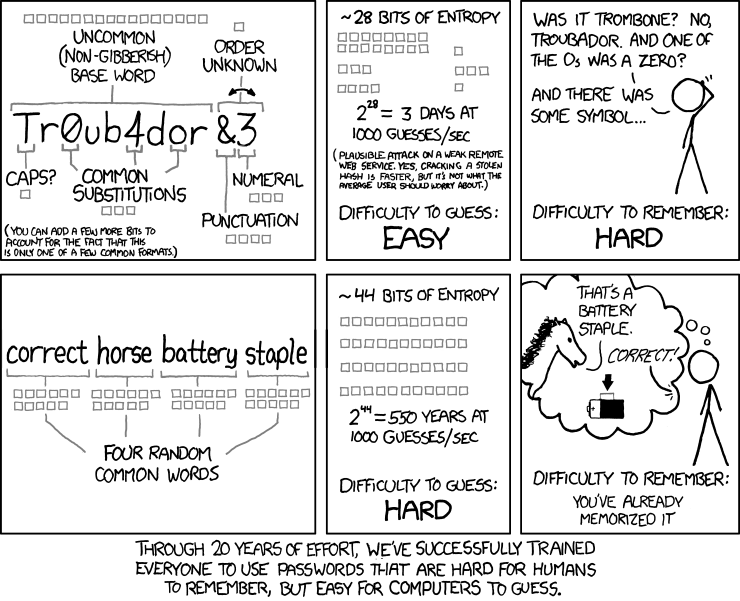
\includegraphics[scale=0.30]{pictures/password_strength.png}
\end{center}
\end{frame}
\begin{frame}{What is a secure password}
A secure password will contain at least 15 characters\\
\end{frame}
\begin{frame}{Passphrases over passwords}
Phrases are easier to remember than a random sequence\\
\textbf{More secure too}
\end{frame}
\begin{frame}{Where are  specially important strong passwords}
Full disk encryption
Password manager
\end{frame}
\begin{frame}{Password hygiene}
You should change your password on a regular basis\\
Don't reuse the same password, or a modification of them\\
\end{frame}
\begin{frame}{Passwords are personal}
\textbf{Don't share your password}\\
If you have a common service use a different account for each member\\
If that's not possible generate a long random pass-phrase for that specific case\\
\end{frame}
\subsection{Generating secure passwords}
\subsubsection{General  tips}
\begin{frame}{General  tips}
Use words rather than characters\\
Use words in many languages\\
Use proper names\\
Use numbers and symbols
\end{frame}
\subsubsection{Diceware generation}
\begin{frame}{Diceware generation}
\begin{center}
Roll 5 dices, do it 7 times, check the list\\
Get your new password !
\end{center}
\end{frame}
\begin{frame}{There is no 100\% secure}
\href{https://archive.org/details/how-to-make-a-super-secure-password}{How To Make A Super-Secure Password}
\end{frame}
\begin{frame}{How to generate passwords}
\begin{enumerate}
\item Search diceware word list \href{https://www.eff.org/files/2016/07/18/eff_large_wordlist.txt}{EFF has a good one}\\
Download the file and avoid search
\item Roll 5 dices and note the number of each dice (ex. 1,5,3,4,2 (15342))
\item Search the equivalent word that correspond to that number
\item Repeat it 6 times for standard password and 7+ for your more important ones
\end{enumerate}
\end{frame}
\section{How to store passwords}
\begin{frame}{Do I have to remember all of them?}
NO!
\end{frame}
\begin{frame}{Password managers}
Tools designed to store your passwords encrypted using a master password.
\end{frame}
\begin{frame}{There is no 100\% secure}
Single point of failure, if it's compromised  = Game Over :(
\end{frame}
\begin{frame}{Password managers on the cloud}
Some provider allow you to synchronize on the cloud\\
Easier to use across multiple devices\\
They \textbf{WILL} know which service to use and when\\
They \textbf{MAY} know your password
\end{frame}
\subsection{KeePassX}
\begin{frame}{KeePassX}
"KeePassX is an application for people with extremly high demands on secure personal data management." - \href{https://www.keepassx.org/}{KeePassX}\\
\begin{center}
Free\\
Open Source\\
Multi platform
\end{center}
\end{frame}
\begin{frame}{Database}
Where passwords are stored\\
Each database is protected by a password, key file, or both
\end{frame}
\begin{frame}{Something you know: Master password}
It has to be strong\\
You have to remember it
\end{frame}
\begin{frame}{Something you have: Key file}
\begin{center}
A file on external storage\\
\begin{tabular}{cc}
\\
\textbf{For} & \textbf{Against} \\
Harder to guess & Like a physical key\\
than a password (usually)&if you lose you are fucked\\ 
\end{tabular}
\end{center}
\end{frame}
\begin{frame}{Combination: password+key file}
Use both of them!
Think about your thread model
\end{frame}
\subsubsection{Let's use it}
\begin{frame}{Creating a database}
In order to create a database:\\
Select new database from the menu (Database / New Database)\\
Specify your password / key file / both\\
If you want you can create multiple  databases with different passwords\\
Any file can be used  as a key file, as long as you don't modify that copy of it\\
Ex. one for the internet, another for work-related  and a third for banking information
\end{frame}
\begin{frame}{Organizing your passwords}
Each database can include groups and these groups can include groups, and...\\
Each group  represent a category of passwords\\
They don't add  any security\\
Ex. social networks, email...
\end{frame}
\begin{frame}{Creating passwords}
Right click on the desired group > Add new entry\\
Enter the title\\
Enter the password to save (you can generate a random password)\\
Fill the additional information\\
Click OK
\end{frame}
\begin{frame}{Generating a random password}
Desired character set\\
You don't need to remember it (unless you loss the password manager)\\
Use it to generate longer passwords
\end{frame}
\begin{frame}{Why are we doing this? Using the password}
You select the password / Right click / Copy password to clipboard
\end{frame}
\begin{frame}{Other features}
\begin{itemize}
\item Search
\item Lock
\item It can store anything you write on the password field (dates, serial numbers...)
\end{itemize}
\end{frame}
\subsubsection{On mobile}
\begin{frame}{Compat}
Android : KeePassDroid\\
iOS:  MiniKeePass\\
\begin{center}
Free\\
Open Source\\
\end{center}
\end{frame}
\begin{frame}{Compatible}
You can use the same password file\\
Mobile devices are less secure, copy just the passwords you will need when you are outdoors
\end{frame}
\end{document}
